\documentclass[letter]{article}
\renewcommand{\baselinestretch}{1.25}

\usepackage[margin=1in]{geometry}
\usepackage{physics}
\usepackage{amsmath}
\usepackage{graphicx}
\usepackage{hyperref}


% MATLAB Formating Code
\usepackage[numbered,framed]{matlab-prettifier}
\lstset{style=Matlab-editor,columns=fullflexible}
\renewcommand{\lstlistingname}{Script}
\newcommand{\scriptname}{\lstlistingname}

\allowdisplaybreaks

%opening
\title{MECH 6313 - Homework 1}
\author{Jonas Wagner}
\date{2021, February 1}

\begin{document}

\maketitle


\section{Problem 1 - Duffing's Equation}
Duffings Equation is exhibits chaotic behavior with certain parameters. It is discribed by the following:
\begin{displaymath}
	\ddot{y} + \delta \dot{y} - y + y^3 = \alpha \cos(\omega_t t)
\end{displaymath}

\textbf{Problem:}
Simulate the equation for $\delta = 0.05, \alpha = 0.4$, and $\omega_t = 1.3$.\\

\textbf{Solution:}
In matlab the nlsys class (something I have been developing to help in nonlin system simulation - \href{https://github.com/jonaswagner2826/nlsys}{https://github.com/jonaswagner2826/nlsys}) was used to simulate the system and plot the following phase plots and time responses. The MATLAB code for this assignment is available in \appendixname \ref{script:HW1}\\



\begin{figure}[h]
	\centering
	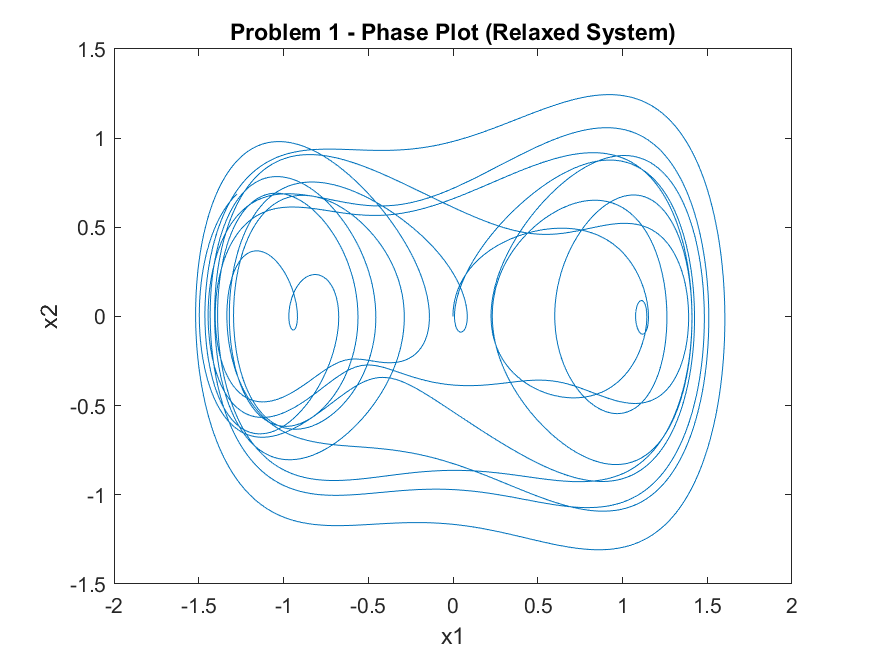
\includegraphics[width=0.7\linewidth]{fig/pblm1_phase}
	\caption{Phase Plot for the Relaxed System}
	\label{fig:pblm1phase}
\end{figure}


\begin{figure}[p]
	\centering
	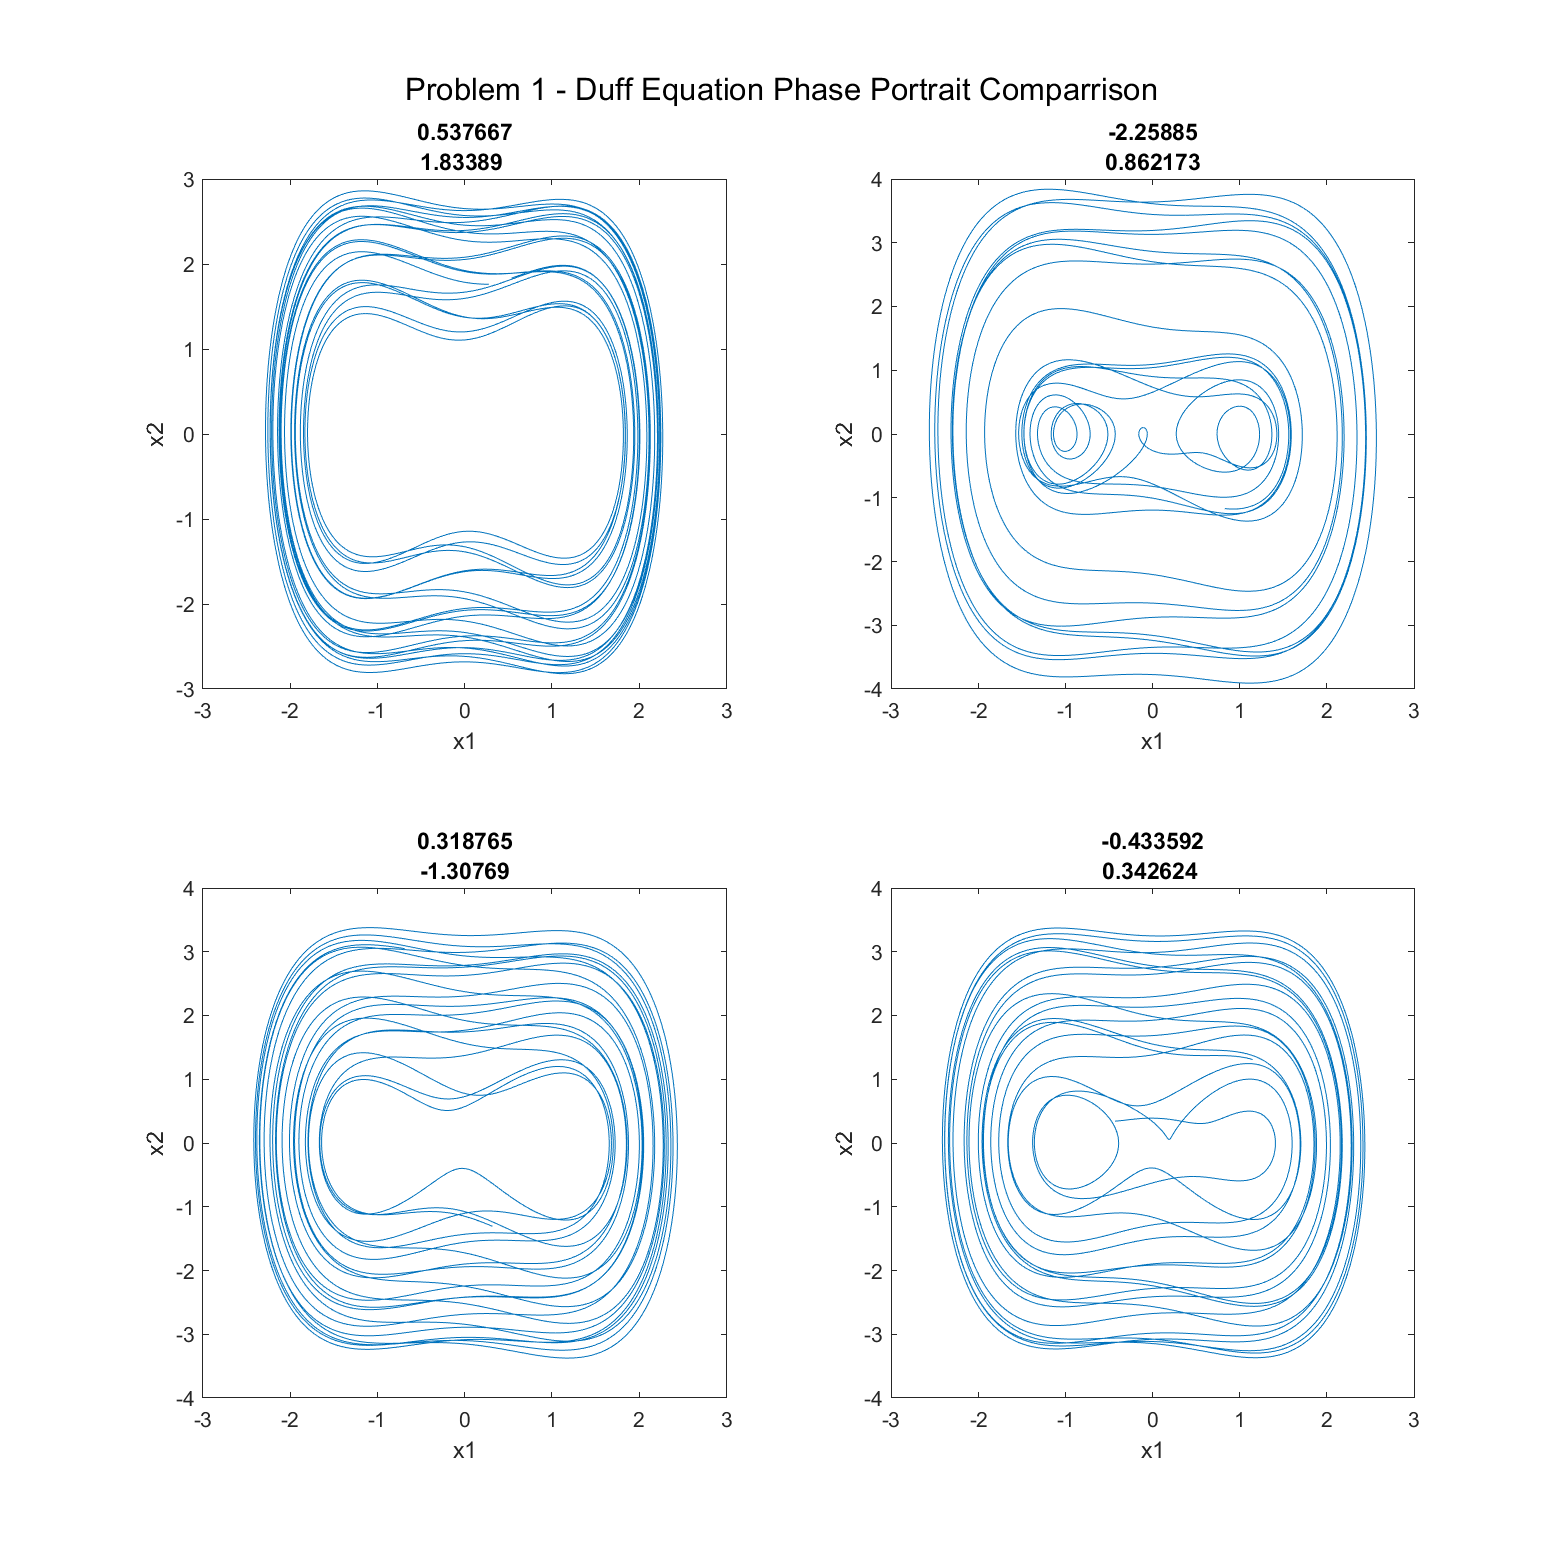
\includegraphics[width=1\linewidth]{fig/pblm1_phase_comparrision}
	\caption{Phase Plot for multiple initial conditions}
	\label{fig:pblm1phasecomparrision}
\end{figure}

\newpage
\begin{figure}[t]
	\centering
	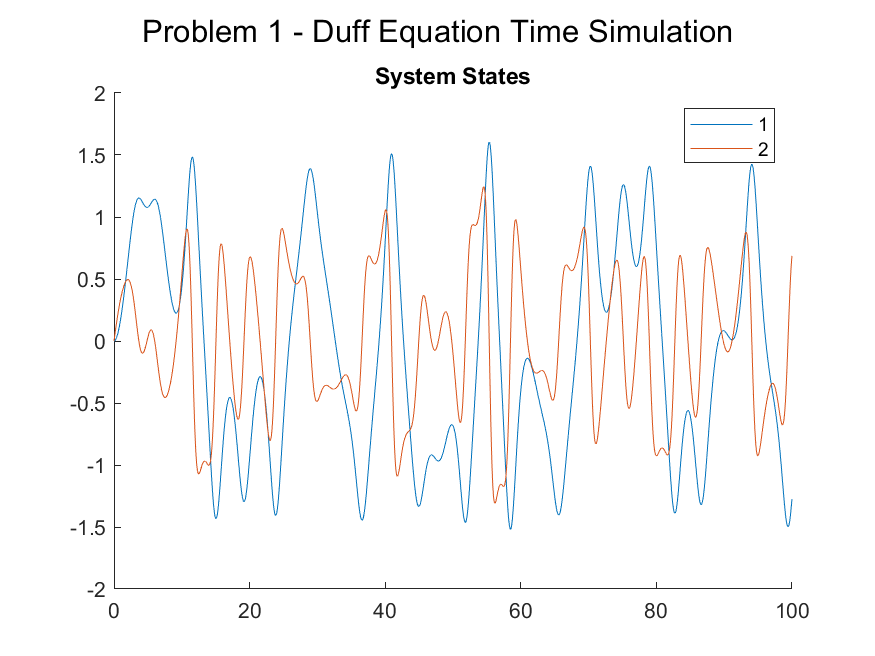
\includegraphics[width=0.8\linewidth]{fig/pblm1_vs_time}
	\caption{Plot of the relaxed system vs time}
	\label{fig:pblm1vstime}
\end{figure}


\textbf{Discussion:}\\

Both the phase portraits and time response of the Duffings equation indicate a fairly chaotic behavior, however it does appear to contentiously rotate around the origin in a periodic fashion (possibly due to the sinusoidal input). Either way, it is difficult to recognize a predictable behavior, and neither decays or explodes predictably.


\newpage
\section{Problem 2 - Van Der Pol Equations}
\textbf{Problem:}
The van der Pole equation is as follows:
\begin{displaymath}
	\ddot{y} + \qty(y^2 - 1)*\dot{y} + y = 0
\end{displaymath}

Plot the phase portrait, time dependence and compare with the response of Duffing's equations.\\

\textbf{Solution:}
In matlab the nlsys class (something I have been developing to help in nonlin system simulation - \href{https://github.com/jonaswagner2826/nlsys}{https://github.com/jonaswagner2826/nlsys}) was used to simulate the system and plot the following phase plots and time responses. The MATLAB code for this assignment is available in \appendixname \ref{script:HW1}

\subsection{Van Der Pol Simulation}

\subsubsection{Phase Portraits}

\begin{figure}[h]
	\centering
	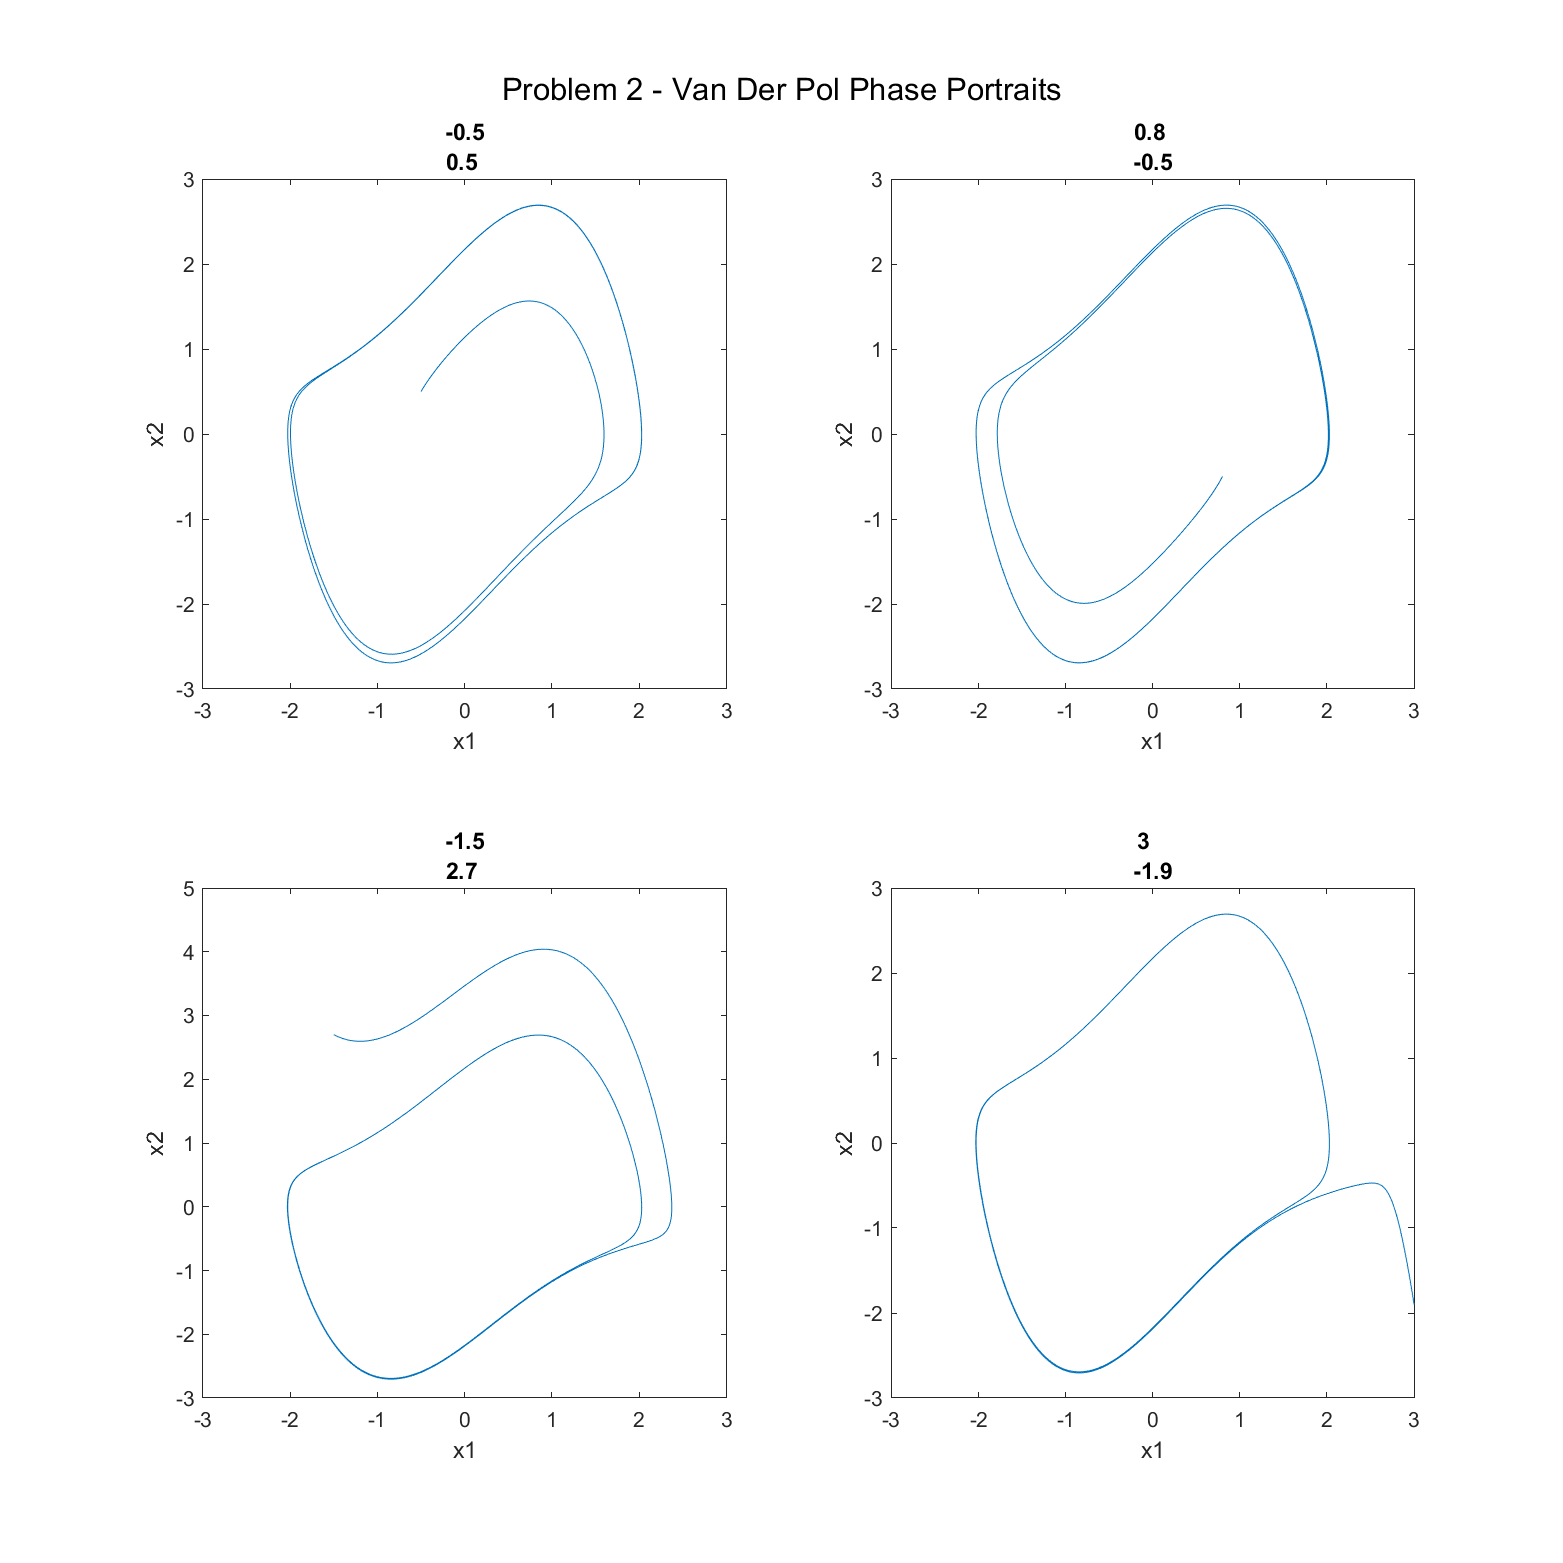
\includegraphics[width=0.8\linewidth]{fig/pblm2_phase_comparrision}
	\caption{Phase Plot for multiple initial conditions}
	\label{fig:pblm2phasecomparrision}
\end{figure}

\newpage
\subsubsection{Time Response}
\begin{figure}[h]
	\centering
	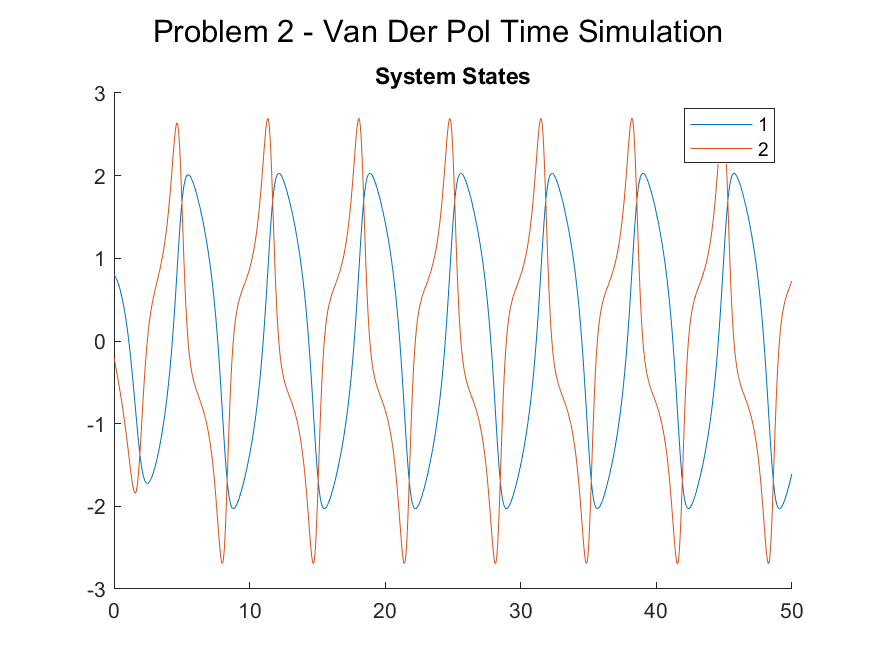
\includegraphics[width=0.8\linewidth]{fig/pblm2_vs_time}
	\caption{Phase Plot for multiple initial conditions}
	\label{fig:pblm2vstime}
\end{figure}


\textbf{Discussion:}

Unlike the results from the duffings equation, the Van Der Pol equations produce a very predictable response. Outside of the equilibrium point located at the origin, the unforced response from any initial equation appears to decay to the exact same periodic motion. Looking at the time response plot, the system states demonstrate a periodic response consistant with expectations from the phase portrait.



\newpage
\subsection{Negative Van Der Pole Equation}

Modifying the nonlinear term of the van der pole equations results in the following differential equation:
\begin{displaymath}
	\ddot{y} - \qty(y^2 - 1)*\dot{y} + y = 0
\end{displaymath}


\subsubsection{System Stability at the Origin}

The Van Der Pol equation can be linearized at the origin by using a taylor's series expansion of the state-space model. The first term can be found by taking the jacobian and evaluating it with $x=\mqty[0&0]^T$.

Letting $x_1 = y$ and $x_2 = \dot{y}$, the following state-space model is derived:
\begin{displaymath}
	\vb{\dot{x}} = f(\vb{x},\vb{u}) = \mqty[x_2 \\ -(x_1^2 - 1) x_2 - x_1]
\end{displaymath}

The jacobians for the $A$ matrix can then be found as:
\begin{align*}
	A 	&= \eval{\mqty[\dv{f_1}{x_1}& \dv{f_1}{x_2}\\ \dv{f_2}{x_1} & \dv{f_2}{x_2}]}_{\vb{x}= \vb{x}_0}\\
		&= \eval{\mqty[0 & 1\\ -2 x_1 x_2 -1 & -x_1^2 +1]}_{\vb{x} = \vb{x}_0}\\
		&= \mqty[0 & 1 \\ -1 &1]
\end{align*}

The stability of this matrix can then be determined by looking at the eigenvalues:
\begin{displaymath}
	\Lambda\{A\} = 0.5 \pm j 0.866
\end{displaymath}

Since $\real\{\Lambda\{A\}\} > 0$, the linearized system is said to be unstable at the origin.

\newpage
\subsubsection{Phase Portraits}

\begin{figure}[h]
	\centering
	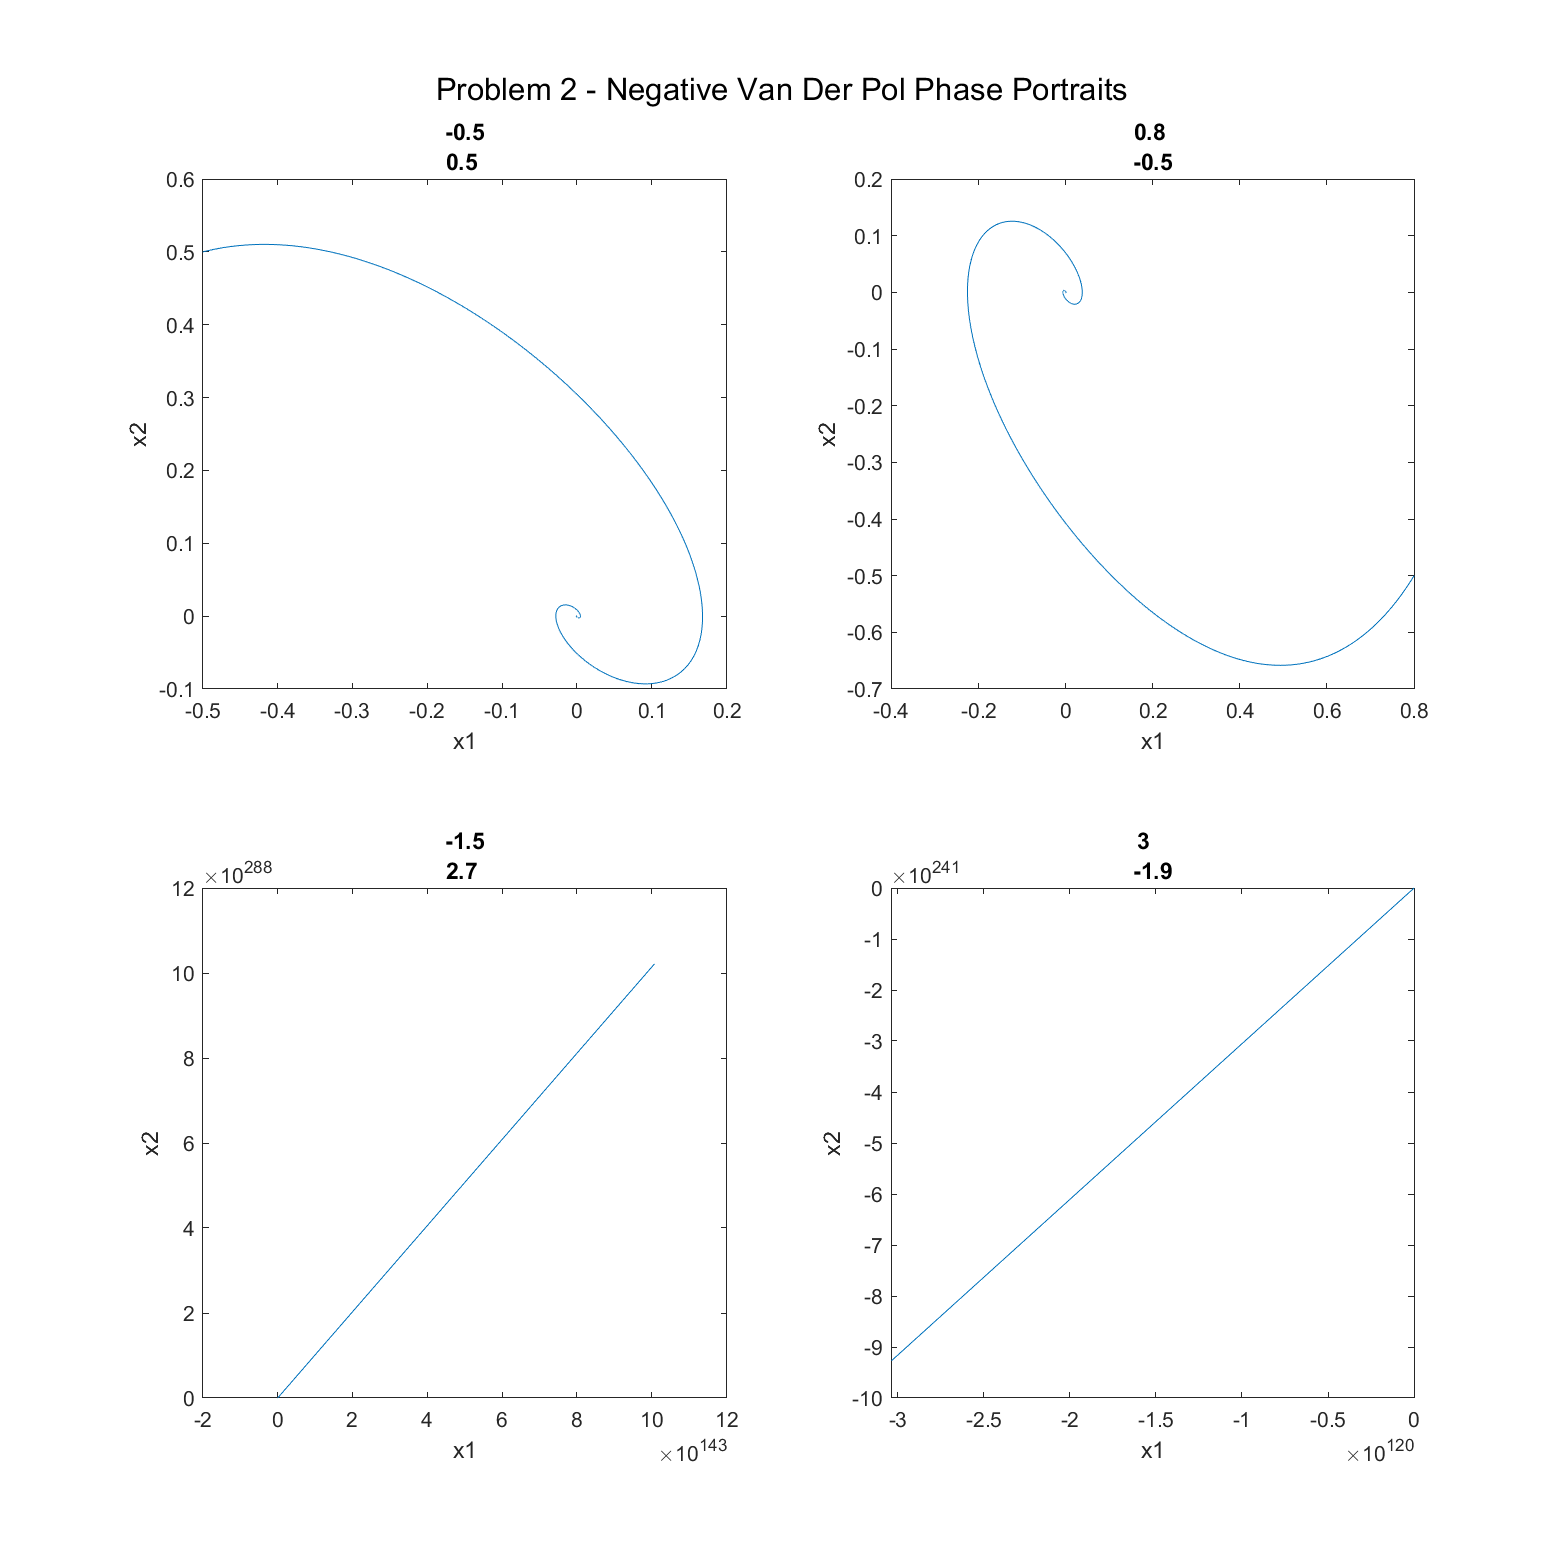
\includegraphics[width=1\linewidth]{fig/pblm2_phase_comparrision_neg}
	\caption{Phase Plot for multiple initial conditions}
	\label{fig:pblm2phasecomparrisionneg}
\end{figure}

\newpage
\subsubsection{Time Response}
\begin{figure}[h]
	\centering
	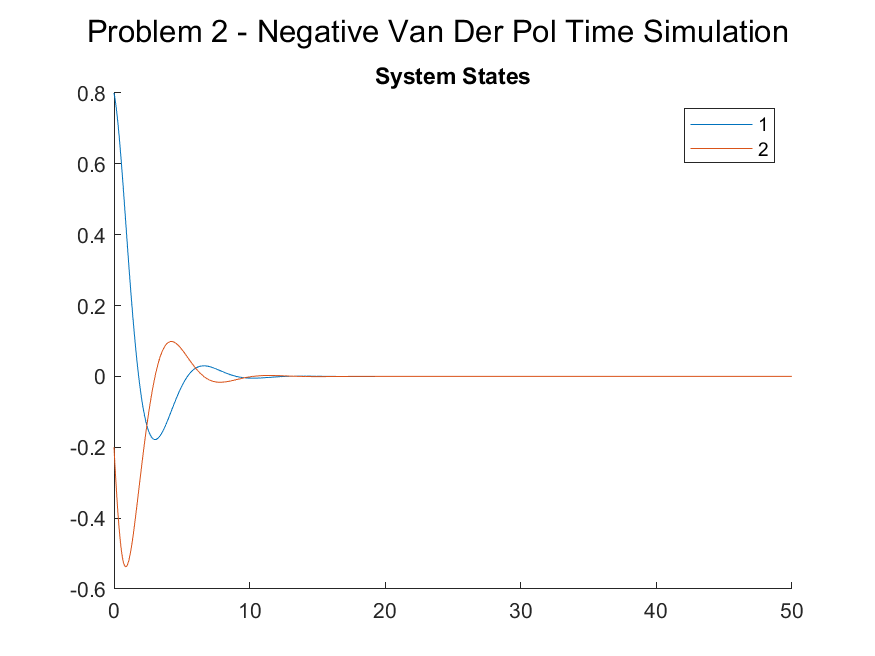
\includegraphics[width=0.8\linewidth]{fig/pblm2_vs_time_neg}
	\caption{Phase Plot for multiple initial conditions}
	\label{fig:pblm2vstimeneg}
\end{figure}


\textbf{Discussion:}
Unlike in the positive van der pol equation, when the nonlinear term is set to be negative it reacts almost directly oposite of the positive one. As was discovered, the origin within the negative system is asymptotically stable, but this is not true in general. From the simulations it is apparent that the same boundary that is the steady-state response for the positve van der pol equation is the boundary of instability. The system is indead localy stable within that boundary and decays to zero, but outside it blows up. It actually doesn't blow up exactly as expected either, depending on the initial condition it won't necessarily just explode out to the extremes of its own quadrant but instead it changes with the initial condition.


\newpage
\appendix
\section{MATLAB Code:}
All code I write in this course can be found on my GitHub repository:\\
\href{https://github.com/jonaswagner2826/MECH6313}{https://github.com/jonaswagner2826/MECH6313}
% MECH6313_HW1
\lstinputlisting[caption={MECH6313\_HW1},label={script:HW1}]{MECH6313_HW1.m}


\end{document}
